\chapter{Prehľad algoritmov}
Na hľadanie najkratších ciest v grafe poznáme mnoho algoritmov, ktoré vieme rozdeliť do troch skupín.


\begin{itemize}
\item Point To Point Shortest Path(P2PSP) - hľadajú najkratšiu cestu medzi dvoma zadanými bodmi
\item Single Source Shortest Path(SSSP) - pre daný vrchol {\sl v} hľadajú najkratšiu cestu do všetkých vrcholov grafu.
\item All Pairs Shortest Path (APSP)- skúmajú najkratšiu cestu medzi všetkými dvojicami vrcholov.
\end{itemize}

Napriek tomu, že sú tieto problémy na obecných grafoch NP-ťažké, na mriežkových grafoch, kde majú všetky vrcholy kladnú cenu, vieme nájsť riešenie v polynomiálnom čase.
V práci sa budeme ďalej zaoberať riešením prvého problému (Point to Point Shortest Path). 

V tejto kapitole si popíšeme algoritmy, ktoré sú použiteľné na všetkých grafoch 
s nezápornými dĺžkami hrán.

\section{Dijkstrov algoritmus}
Medzi základné algoritmy typu SSSP patrí Dijkstrov algoritmus \ref{alg:dijkstra} popísaný už v roku 1959.
Patrí medzi relaxačné algoritmy a jeho činnosť si vieme predstaviť ako posúvanie vlny po grafe TODO??WTf did I just write?


Pri hľadaní cesty z vrcholu $s$ do vrcholu $t$ prechádzame postupne vrcholy zo stúpajúcou vzdialenosťou od $s$, až dokým sa nedostaneme k cieľovému vrcholu $t$.
Vizuálne si beh algoritmu môžme predstaviť ako kruh so stredom v bode $s$ so zväčšujúcim sa polomerom.

Algoritmus je nasledovný \ref{alg:dijkstra}. 
?? rozlisujeme tri stavy vrcholov, co je halda blablabla
ASK??ako odkazovat?

FIXME ?? kolize H a h()
\begin{algorithm}
\caption{Dijkstra: nájdi najkratšiu cestu medzi dvoma bodmi $s$ a $t$}
\label{alg:dijkstra}
\begin{algorithmic}[1] % number one = line numbering is on
\REQUIRE graf $G$
\ENSURE hodnotiaca funkcia $h$ obsahujúca najkratšie cesty  z vrcholu $s$ do vrcholov grafu


\STATE $ h(*) \leftarrow \infty $
\STATE $ stav(*) \leftarrow$ NENAVŠTÍVENÝ

\COMMENT {pridám počiatok}
\STATE $h(s) \leftarrow 0$
\STATE $stav(s) \leftarrow $ OTVORENÝ
\STATE Heap $H$
\STATE $Insert(H, s)$

\WHILE {$H$  not empty}
	
	\STATE // vyberiem v -- najbližší otvorený vrchol
	\STATE $v \leftarrow ExtractMin(H)$
	
	\WHILE {$stav(v) \neq $ OTVORENÝ}
		\STATE $v \leftarrow ExtractMin(H)$
	\ENDWHILE
	
	\STATE // zrelaxujeme vrchol $v$
	\FORALL {$e$, $e = (v, u)$}
		\IF {$h(u) \textgreater h(v) + l(v, u)$}
			\STATE $Insert(H, v)$
			\STATE $stav(u) \leftarrow$ OTVORENÝ
			\STATE $h(u) \leftarrow h(v) + l(v, u)$
			
		\ENDIF
	\ENDFOR
\ENDWHILE

\end{algorithmic}
\end{algorithm}

\begin{theorem}
V dijkstrovom algoritme uzatvárame každý dosiahnuteľný vrchol práve raz.
\end{theorem}
ASK?? citovat dijkstru a maresa ako dokaz? 

\subsection{Zložitosť}
popis len obecne pomocou casu na ExtractMin a Insert.


\section{Lineárny Dijkstrov algoritmus}
Zložitosť vyššiepopísaného algoritmu \ref{alg:dijkstra}
závisí od haldy, ktorú použijeme. Pri použití binárnej haldy bude \BigO{blablabla}.TODO??

Nakoľko pre mriežkový graf platia ....??

\begin{theorem}
Pokiaľ sme v Dijkstrovom algoritme uzavreli vrchol $u$ so vzdialenosťou $d_u$ a najkratšia hrana v grafe má dĺžku $\epsilon$, tak môžme taktiež 
uzavrieť všetky vrcholy $v$ so vzdialenosťami $d_v \in (d, d + \epsilon)$.
\end{theorem}
\begin{proof}
Do haldy vieme pridávať len vrcholy so vzdialenosťami aspoň $d + \epsilon$ (kratšia hrana tam už nie je), 
ale~tie už cestu k~vrcholom so~vzdialenosťami
$d_v \in (d, d + \epsilon)$ skrátiť nemôžu.
\end{proof}



Keďže veľkosť najkratšej hrany $\epsilon = 1$, tak v štruktúre budeme mať priehradky, ktorých rozsah je ostro menší ako $\epsilon$.
Na konštrukciu lineárneho Dijkstrovho algoritmu potrebujeme priehradkovú haldu. Tá vie vybrať  \uv{jeden z najmenších} prvkov.
v konštantnom čase a rovnako ako aj vložiť prvok.

\begin{figure}[h]
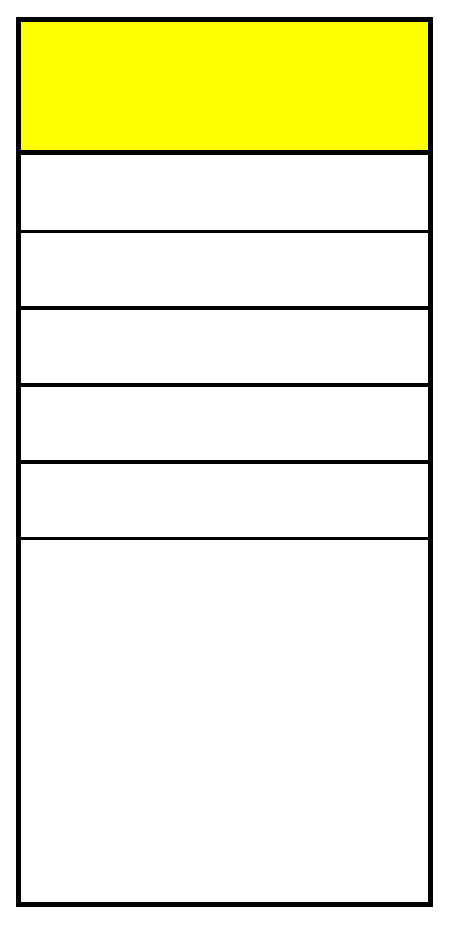
\includegraphics[height=5.5cm]{./img/priehradka.eps}
\caption{Mriežkový graf bez označenia vrcholov a dĺžok hrán}
\label{fig:mriezkovy_graf}
\end{figure}



\section{A*}
dalsi algoritmus do zbierky je a* \cite{astar72}.
